\documentclass[problems]{esg8012exam} 
  \usepackage{amsmath}
  \usepackage{amssymb}
  \usepackage{enumerate}
  \usepackage{graphicx}
  \usepackage{hyperref}
  \usepackage{siunitx}
  \providecommand{\uvec}[1]{{\hat{\bf{#1}}}}
  \usepackage{pgf,tikz}
  \usetikzlibrary{arrows}
  \usepackage{subfigure}
  %\usepackage{wrapfig}
  \newcommand{\subfigureautorefname}{\figureautorefname}
  \makeatletter
  \newcommand{\interitemtext}[1]{%
    \begin{list}{}
     {\itemindent=0mm\labelsep=0mm
     \labelwidth=0mm\leftmargin=0mm
     \addtolength{\leftmargin}{-\@totalleftmargin}}
      \item #1
    \end{list}
  }
  \makeatother
  \renewcommand{\d}{\,d}
  \providecommand{\norm}[1]{\lVert#1\rVert}
\classname{Physics 8.012} 
\semester{Fall 2010} 
\examnumber{1} 
\date{\today } 
\begin{document}
\section{Problem \thesection\space(30 Points)}
  A car is driving through a green light at $t = 0$ located at $x = 0$ with an initial speed $v_{c, 0} = \SI{12}{\meter\per\second}$.  The acceleration of the car as a function of time is given by
  $$a_c = \begin{cases}
            0 & \text{if }0 < t < t_1 = \SI{1}{\second} \\
            -(\SI{6}{\meter\per\second\cubed})(t - t_1) & \text{if }\SI{1}{\second} < t < t_2
          \end{cases}
  .$$
  A bicycle rider is riding at a constant speed of $v_{b,0}$ and at $t = 0$ is \SI{17}{\meter} behind the car.  The bicyclist reaches the car when the car just comes to rest at time $t_2$.

  \begin{enumerate}[(a)]
    \item Find the time $t_2$ that the car has just come to rest.
    \item Find the speed of the bicycle.
  \end{enumerate}
\section{Problem \thesection\space(30 Points)}
  Two blocks with masses $m_1$ and $m_2$ such that $m_1 \ll m_2$ are connected by a massless inextensible string and a massless pulley as shown in the figure below.  The pulley is rigidly connected to the top of a wedge with angle $\theta$.  The coefficient of friction between the blocks is $\mu$.  The surface between the lower block and the wedge is frictionless.  What are the magnitudes of the acceleration of the two blocks?
  \begin{center}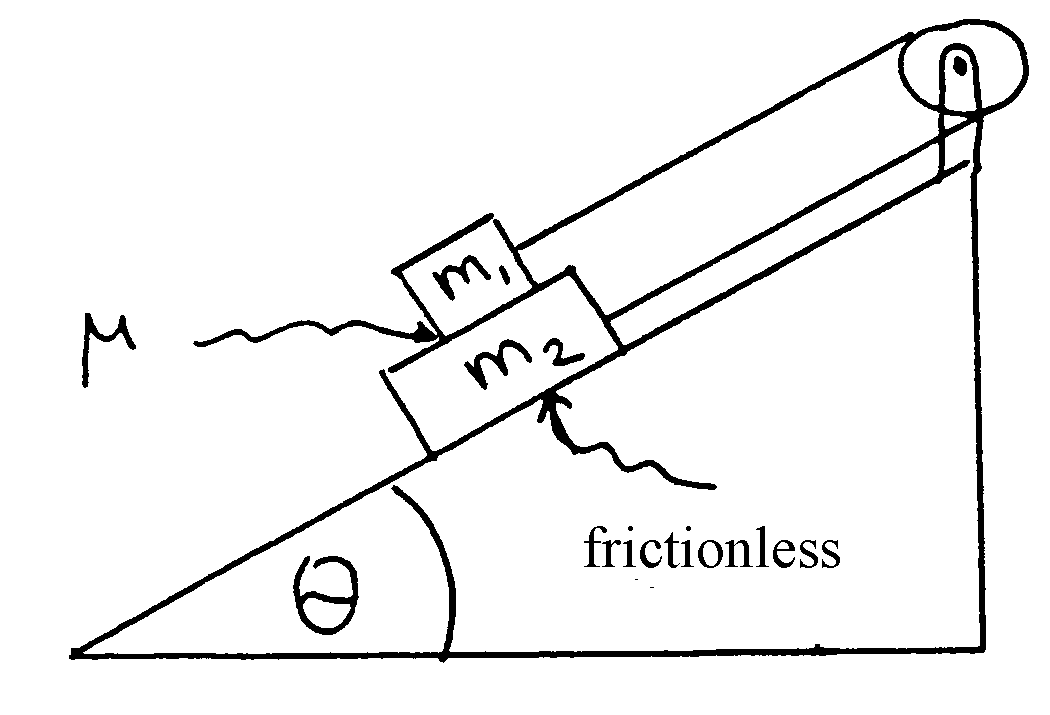
\includegraphics[width=0.33\textwidth]{exam1_p2_1}\end{center}
\section{Problem \thesection\space(30 Points)}
  A U-control airplane of mass $M$ is attached by a wire of length $L$ and negligible mass to the ``pilot'' who controls the ``lift'' provided by the wing, the force that is normal to the plane of the wings keeping the plane aloft and hence in a direction perpendicular to the wire.  The plane's engine keeps it moving at constant speed $v$.  The wire and the wings of the plane make an angle $\theta$ with the ground.  The gravitational acceleration is $g$.  Express your answers to the following questions in terms of $M$, $g$, $L$, $v$, and $\theta$ as needed.
  \begin{enumerate}[(a)]
    \item Find the tension $T$ in the wire when the plane is flown overhead in a circle.
    \item Find a condition that the speed of the plane must satisfy such that, for all values of $\theta$, the tension in the string is not zero. (\textsc{Note}: Your condition should \emph{not} depend on $\theta$.)
    \item Find the magnitude of the ``lift'', the force that is normal to the plane of the wings keeping the plane aloft.
    \item Based on your result form part (c), is $\theta = \pi / 2$ possible?
  \end{enumerate}
  \begin{center}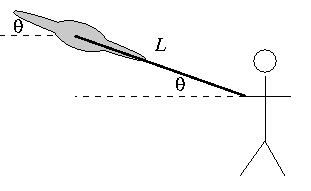
\includegraphics[width=0.4\textwidth]{exam1_p3_1}\end{center}
\section{Problem \thesection\space(10 Points)}
  A bucket of water spins with angular speed $\omega$.  What shape does the water's surface assume.  That is, find an equation for the surface of the water.  Clearly show your coordinate system, free body diagram, and all relevant work.
  \begin{center}
    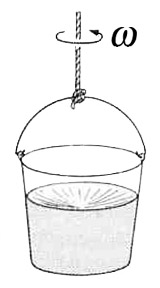
\includegraphics[width=0.18\textwidth]{exam1_p4_1}
  \end{center}
\end{document}
